This chapter addresses the non straightforward problem of computing the fractional part division
% \footnote{explicit base 2 notation}
\begin{equation}
\frac{(1.f_1)}{(1.f_2)}
\end{equation}

When implemented in hardware, different non-negligible trade-offs come into play.

There are three main families of division algorithms \cite{muller_hardware_2010}. 

\begin{itemize}

\item Digit-recurrence (DR) algorithms, such as the family of SRT algorithms named after Sweeney, Robertson, and Tocher, %[344, 408]
generalize the paper-and-pencil algorithm learned at school. They produce one digit of the result at each iteration. Each iteration performs three tasks (just like the pencil-and-paper method): (i) determine the next quotient digit, (ii) multiply it by the divider, and (iii) subtract it from the current partial remainder to obtain a partial remainder for the next iteration.
In binary, there are only two choices of quotient digits, 0 or 1; therefore, the iteration reduces to one subtraction, one test, and one shift. 
A binary digit-recurrence algorithm can therefore be implemented on any processor as soon as it is able to perform integer addition.

One important thing about digit-recurrence algorithms is that they are exact. Starting from fixed-point numbers $X$ and $D$, they compute at iteration $i$ an $i$-digit quotient $Q_i$ and a remainder $R_i$ such that the identity $X = DQ_i + R_i$ holds.
For floating-point purposes, this means that all the information needed for rounding the result is held in the pair $(R_i, Q_i)$.
%In practice, to round to precision $p$, one needs $p$ iterations to compute $Q_p$, then possibly a final addition on $Q_p$ depending on a test on $R_p$.


\item Polynomial approximation can also be used to evaluate $1/x$ to the required accuracy. %[430].
Note that, mathematically speaking, functional iterations evaluate a polynomial in the initial approximation error. % [88].

\item Functional iteration algorithms generalize the Newton Raphson iteration for approximating the function $1/x$. They make sense mostly on processors having a hardware multiplier. The number of iterations is much less than in digit-recurrence algorithms ($\mathcal{O}(\log p)$ versus $\mathcal{O}(p)$), but each iteration involves multiplications and is therefore more expensive. These latter two methods may be combined.
\end{itemize}

\subsection{Approximated reciprocal}

In a quest to discover an alternative route to compute an accurate reciprocate, we came up with the nifty idea of exploiting the Taylor series technique\footnote{the Taylor series of a function is an infinite sum of terms that are expressed in terms of the function's derivatives at a single point. For most common functions, the function and the sum of its Taylor series are equal near this point.} around $ 0.75 = mean([0.5, 1))$.


This seemingly appealing strategy however, hinders a great deal of forthcoming issues, most notably:
\begin{itemize}
\item requires $6$ fixed-point products!\footnote{$3$ due to 3rd-order term $x*x*x*3.1604\dots$ + $2$ + $1$},
\item is only accurate around the close vicinity of the point around which the series is expanded, as shown in figure \ref{fig:relative_error_00001}.
\end{itemize}
A way to circumvent the latter issue comes from employing the Chebyshev polynomials. These are meant to provide the best approximation not around a given point, rather spread across an interval, right what we need.
The better control over the accuracy across the interval is paid in terms of simplicity of calculation (which is out of the scope).


Applying the third order Chebyshev polynomials formula to $1/x$ across the interval $(0.5, 1)$ we obtain
\begin{equation}\label{equ:3rd_order_Chebyshev_polynomial_equation}
f_{cp_3} = 5.65685 - 11.75737x + 10.64818x^2 - 3.54939 x^3 + \mathcal{O}(x^4)
\end{equation}
which, from a qualitative visual inspection (figure \ref{fig:relative_error_00001}) gives the better approximation possible of $1/x$ across the interval, but still suffer from the major problem the Taylor series does, namely the long chain of products.

The breakthrough idea comes from \cite{drom} which \textit{proposes} a fast technique, with the utmost requirement of being suitable for register transfer logic (RTL) implementation, which boils down to the following constraints: (i) no dividers, except power of $2$; (ii) least amount of multipliers; (iii) fixed-point integer arithmetic.


The following routine is indeed hardware friendly, as it employs just two fixed-point multiplications, thsu two integer operations, and a power of $2$ multiplication -- effectively an inexpensive constant bit shift. 

\begin{verbatim}
def reciprocal(a):
    b = 1.466 - a
    c = a * b
    d = 1.0012 - c
    e = d * b
    out = e * 4
    return out
\end{verbatim}


\begin{figure}
    \centering
    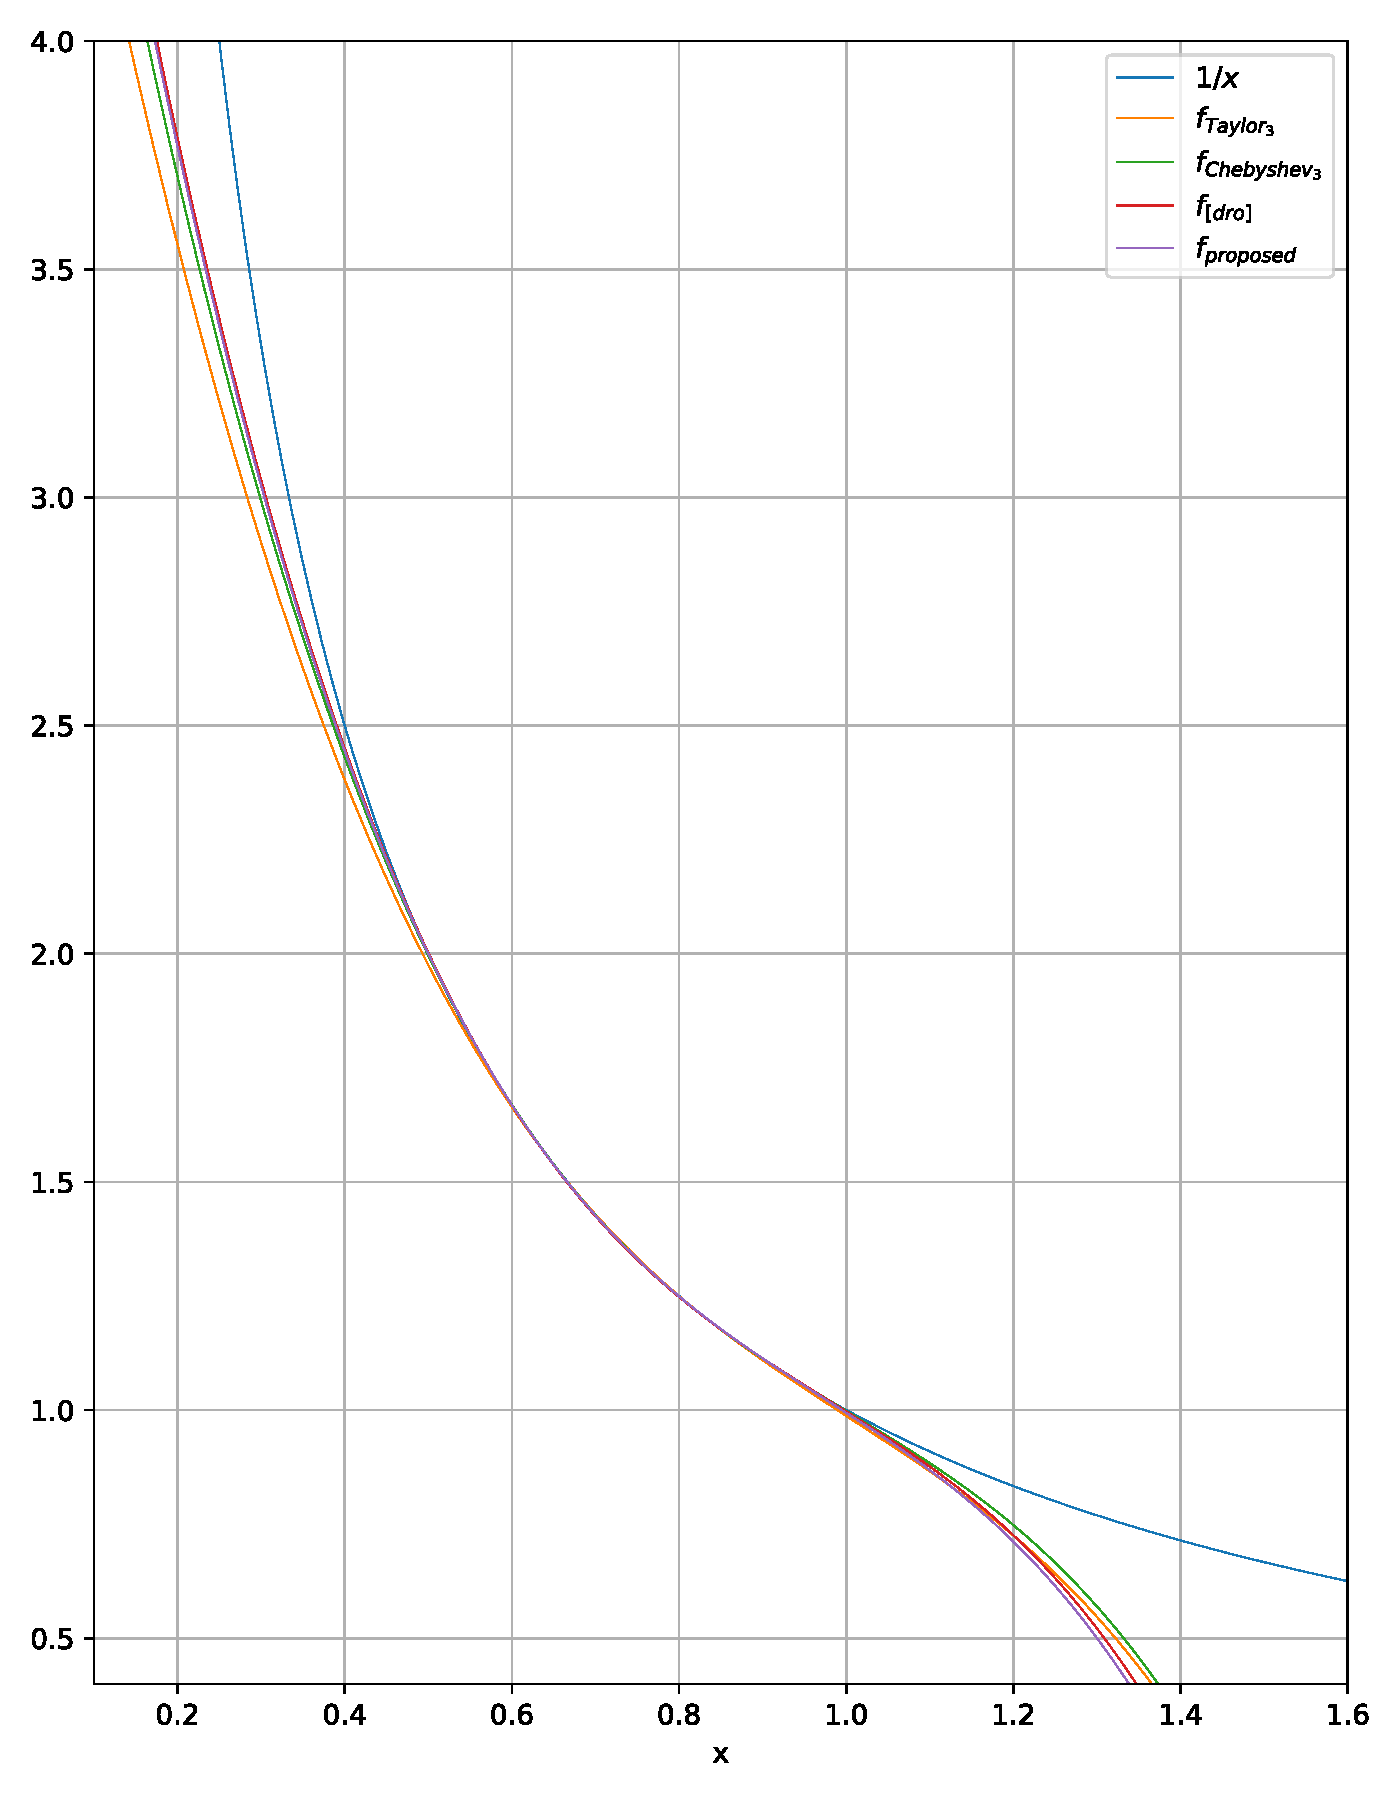
\includegraphics[width=0.75\textwidth]{figures/reciprocate_real_vs_taylor_vs_drom.pdf}
    \caption{Comparison of $1/x$ vs \cite{drom} vs 3rd order Taylor polynomial vs 3rd order Chebyshev polynomial vs proposed solution (i.e. optimized \cite{drom})}
    \label{fig:0203012875432985734}
\end{figure}

\begin{figure}
    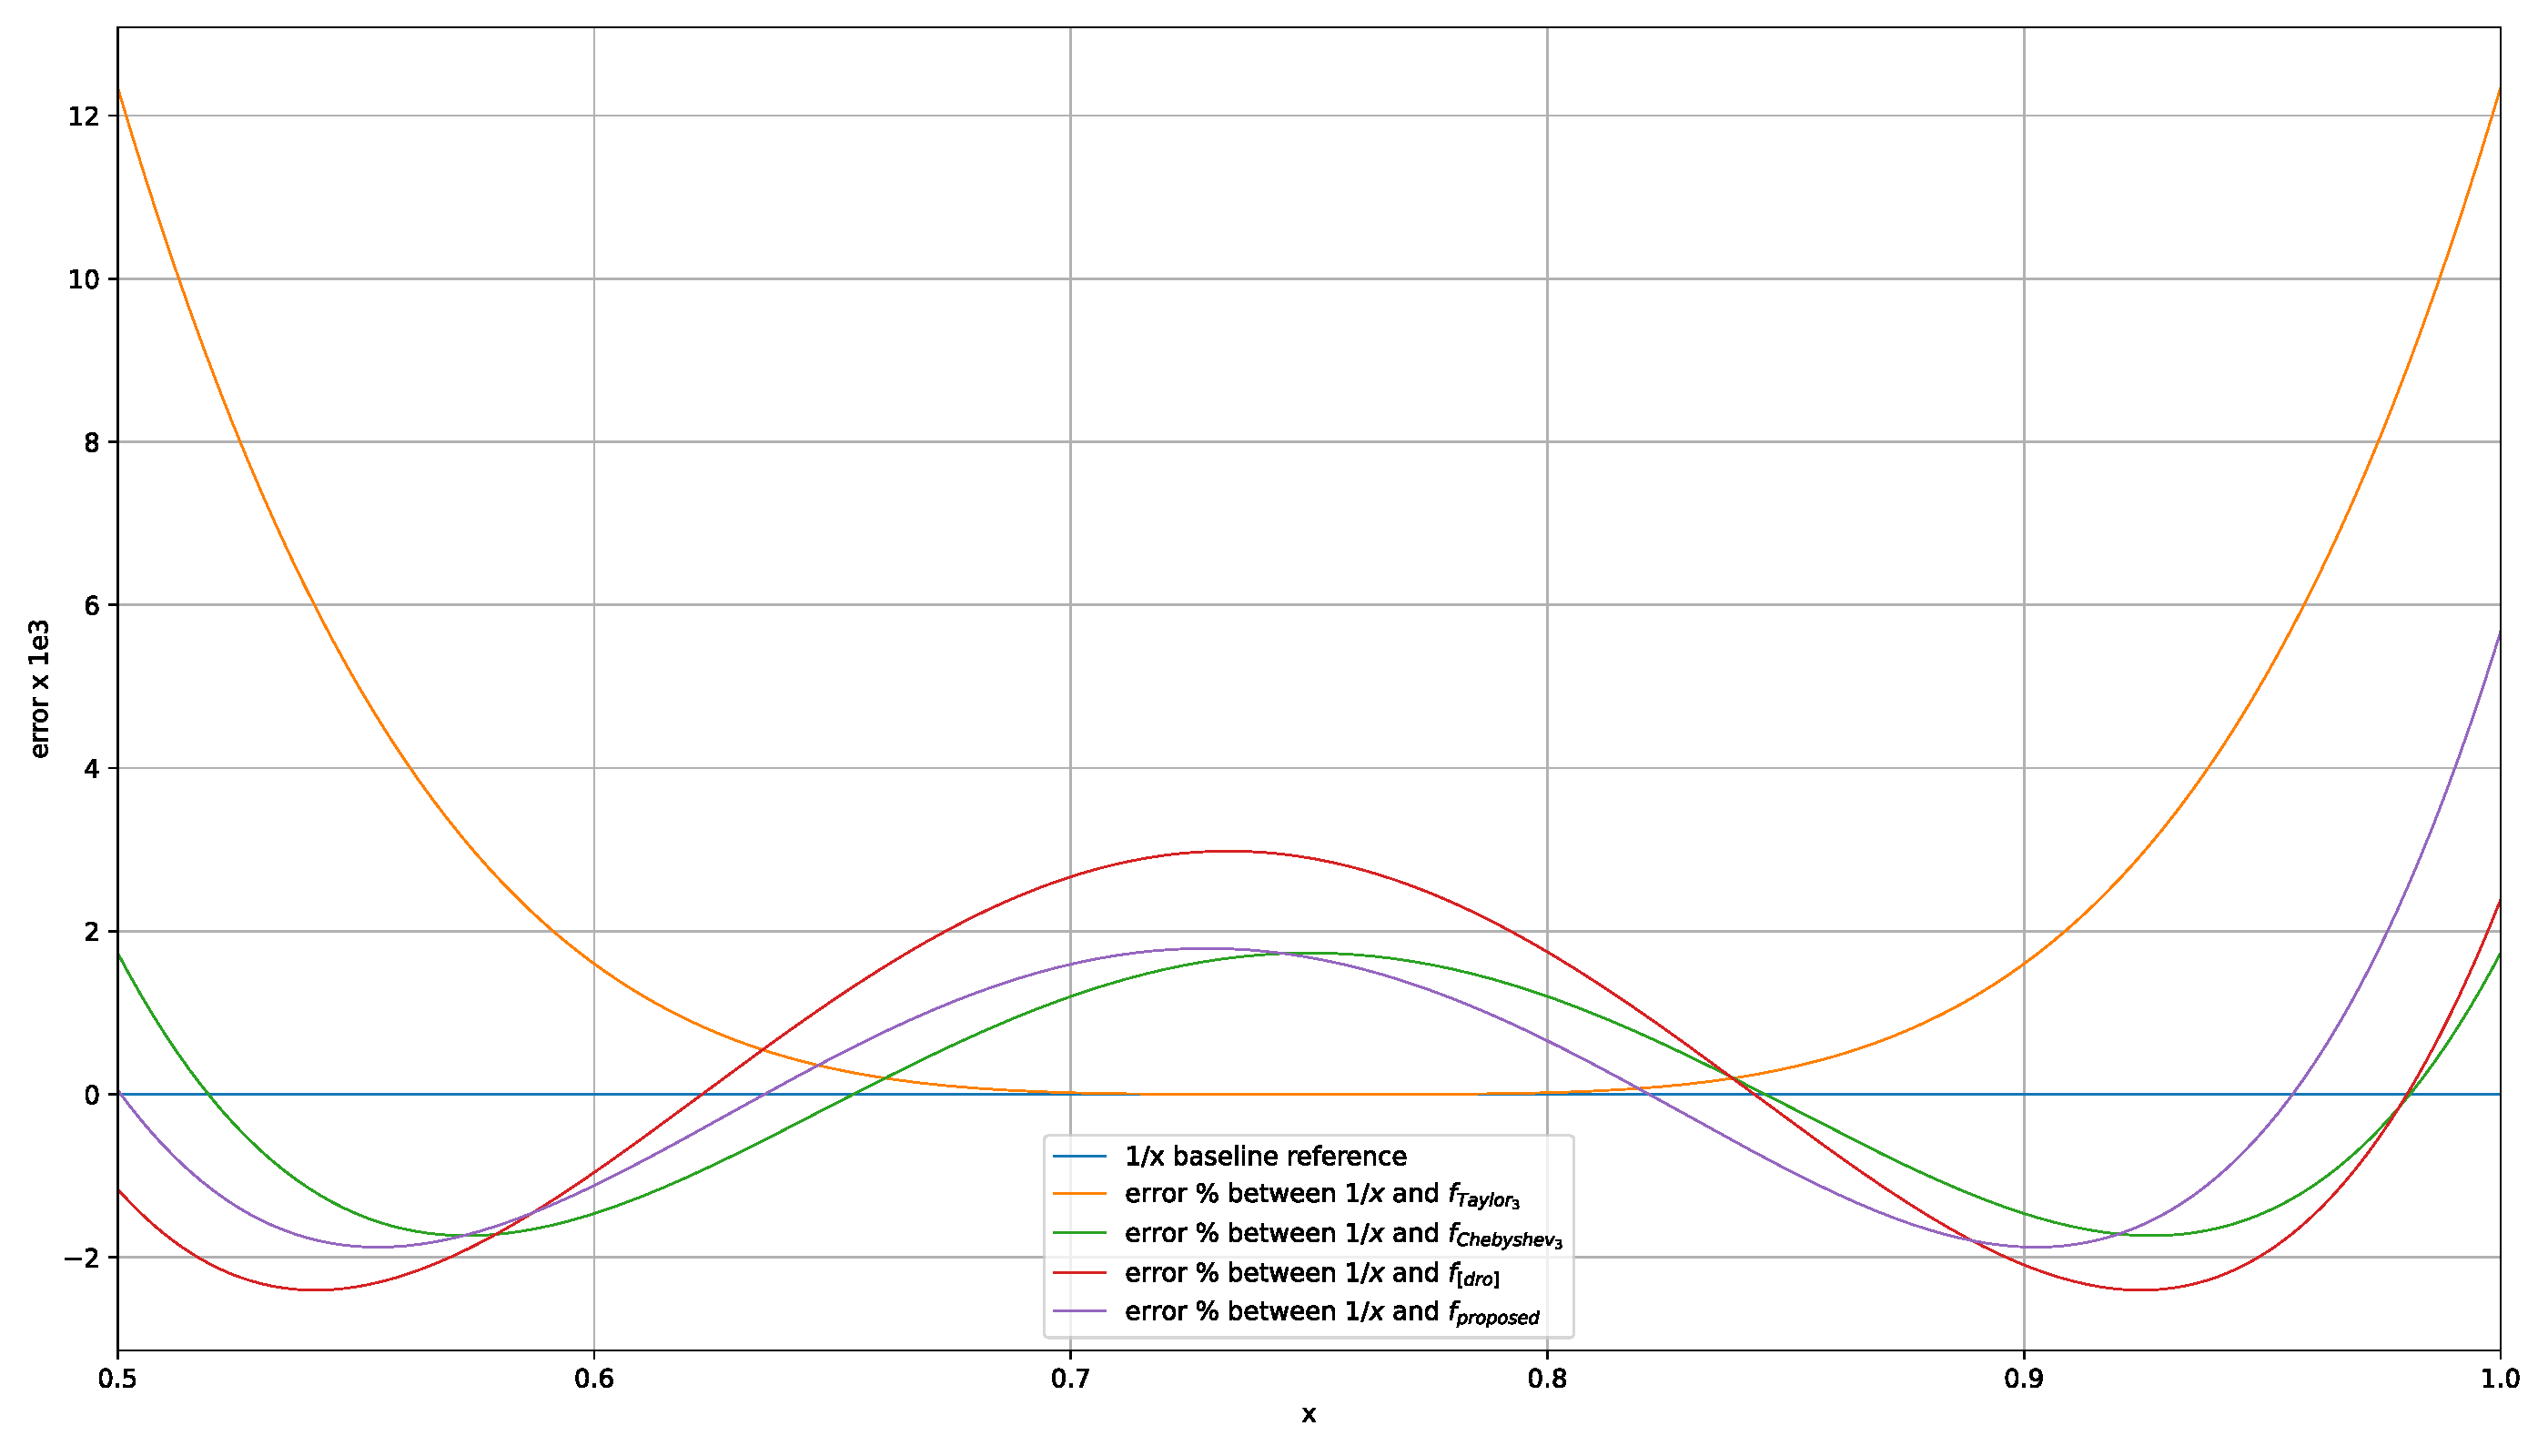
\includegraphics[width=1\textwidth]{figures/reciprocate_real_vs_taylor_vs_drom_error.pdf}\caption{Relative error against reference $1/x$}\label{fig:relative_error_00001}
\end{figure}
\begin{figure}
    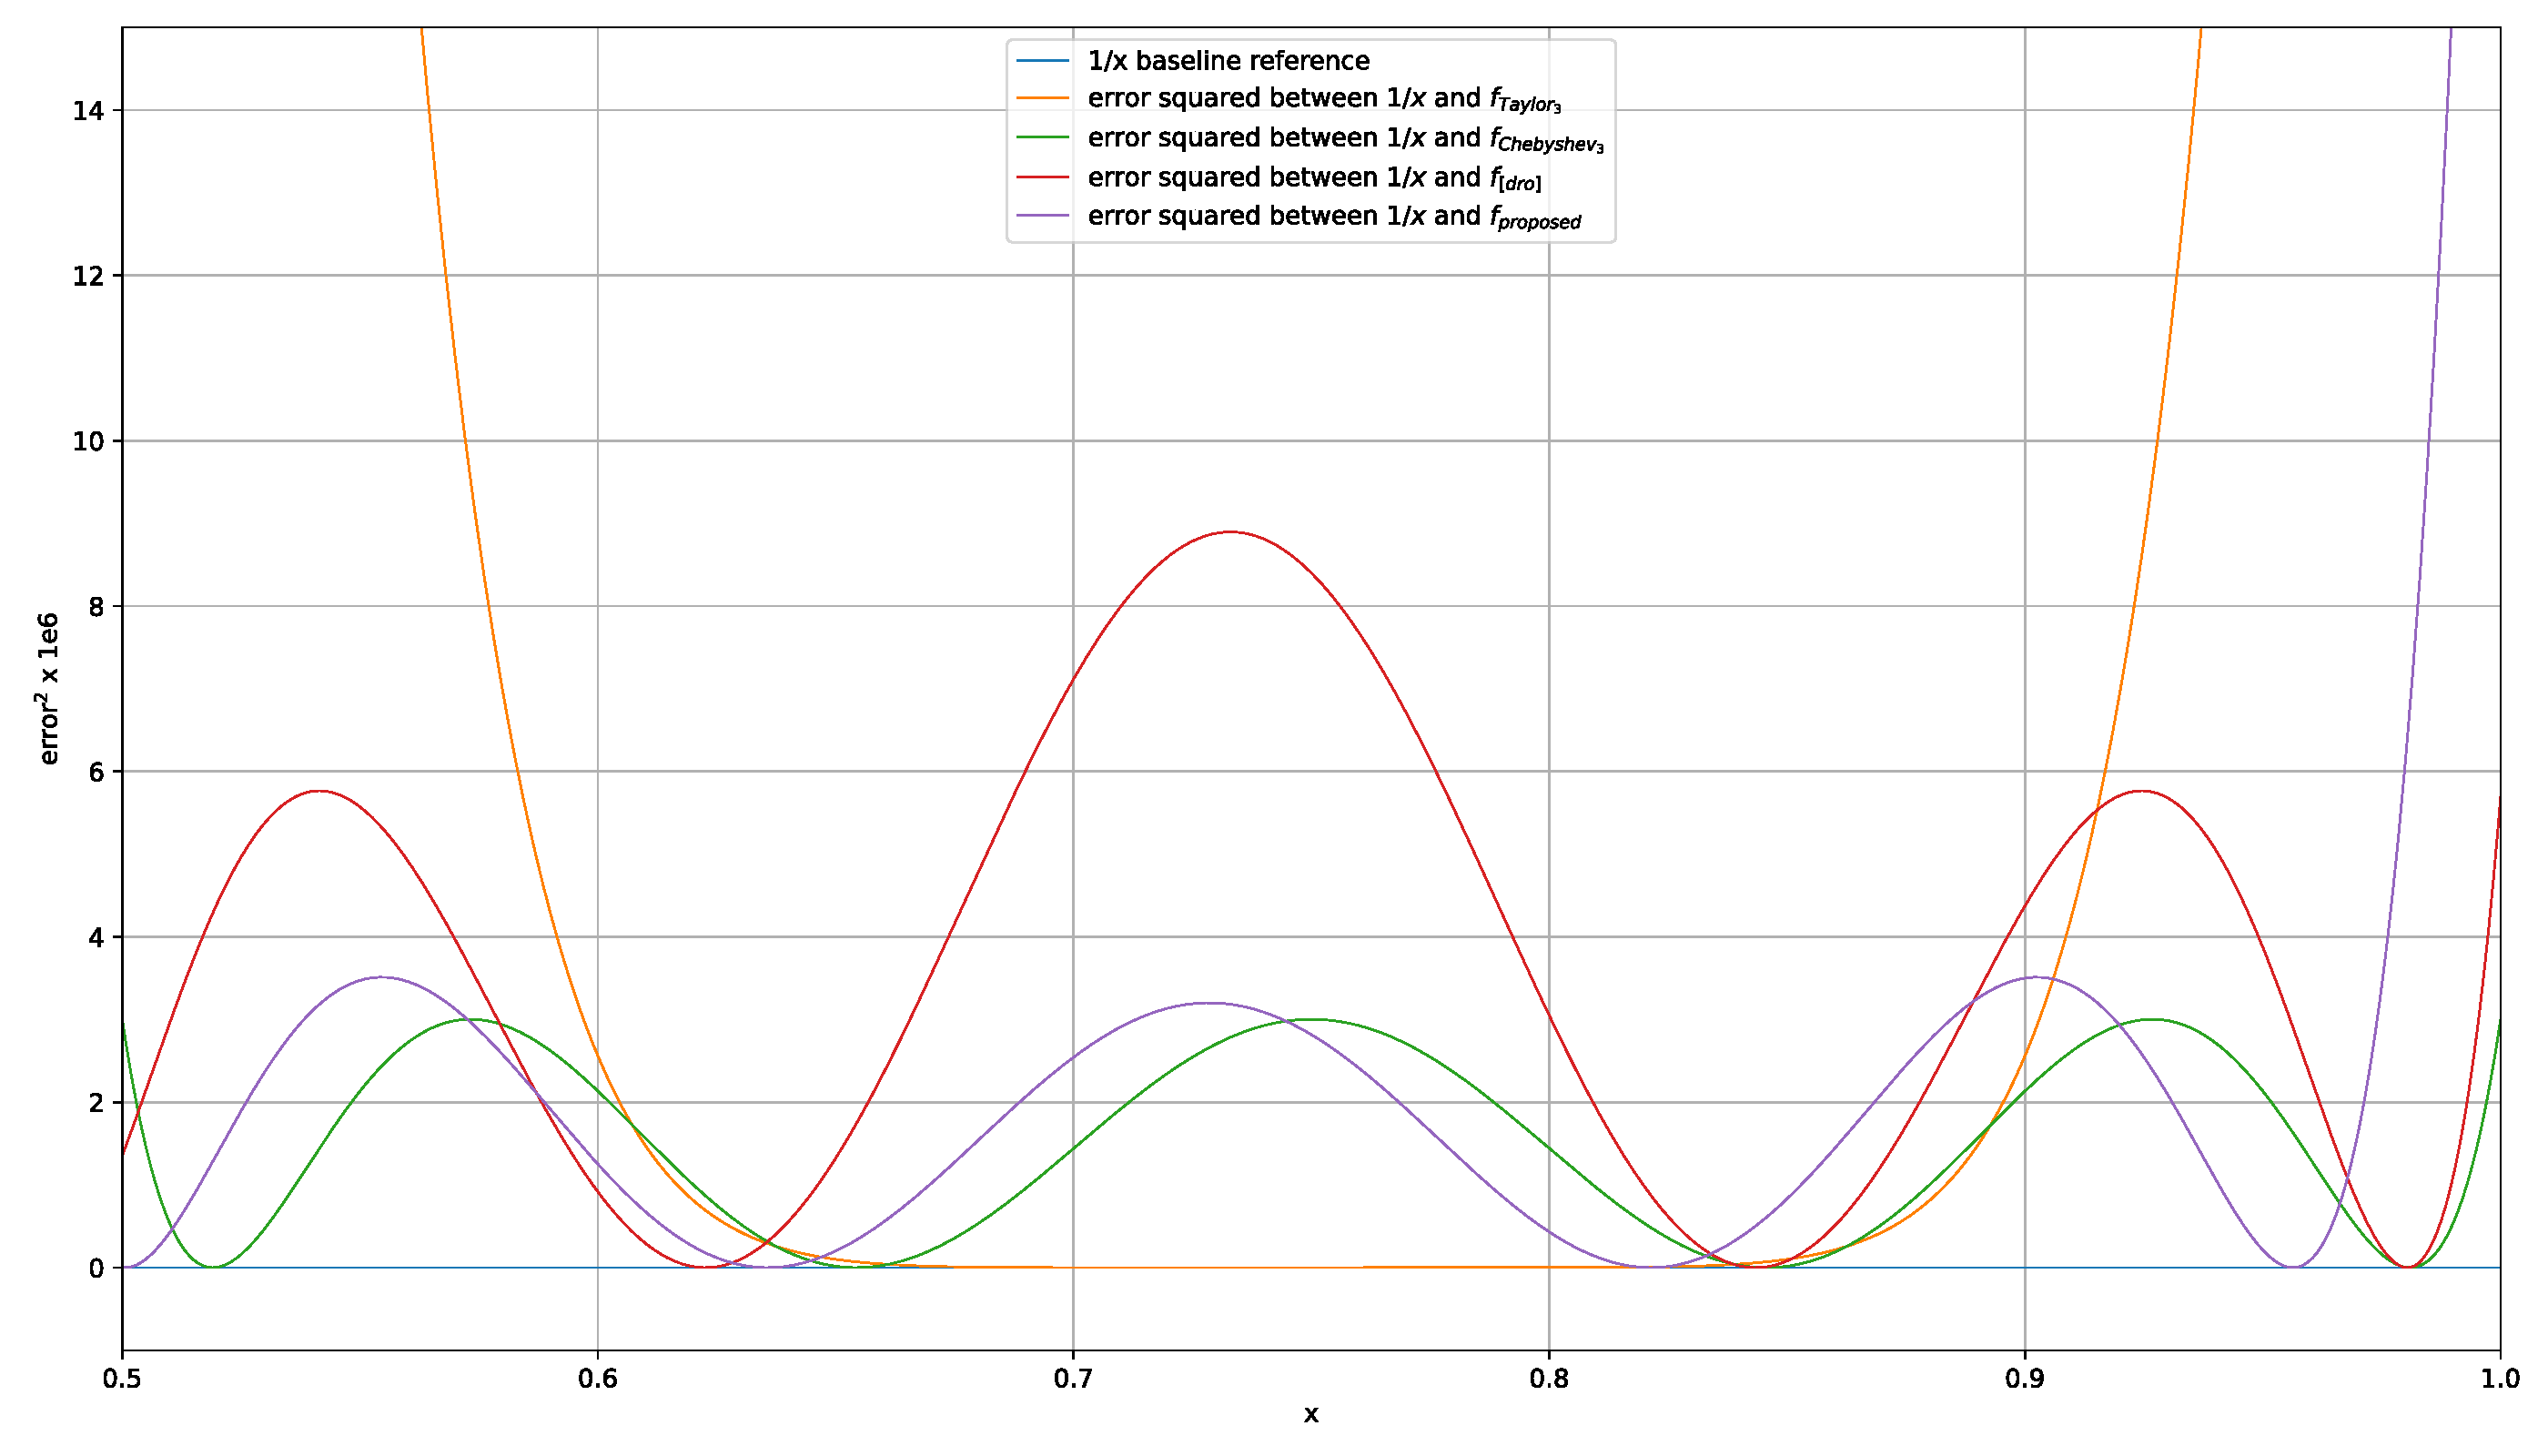
\includegraphics[width=1\textwidth]{figures/reciprocate_real_vs_taylor_vs_drom_error_squared.pdf} 
    \caption{Squared relative error against reference $1/x$}
    \label{fig:020301280980435232835} 
\end{figure} 

Expanding the routine into a full-blown third order polynomial (\ref{equ:expanded_drom_modified_polynomial}, \ref{equ:expanded_drom_0000}) similar to the previous -- generalizing for the two magic numbers\footnote{no explanation provided whatsoever} -- we realize that this is a modified Chebyshev polynomial with the highest grade coefficient pinned at the closest power of two -- $4$ in this case.
This meta-constraint, replaces the need of long chained multiplication required by the \textit{classic} Chebyshev polynomial approximation (\ref{equ:3rd_order_Chebyshev_polynomial_equation}), using just the bare minimum operations, at the bearable price of slightly lower accuracy.
\begin{equation}\label{equ:expanded_drom_modified_polynomial}
\begin{aligned}
f(a, k_1, k_2) &= 4 \cdot e = 4 \cdot d \cdot b = \\
&= 4 \cdot (k_2 - c) \cdot (k_1 - a) = \\
&= 4 \cdot (k_2 - a \cdot b) \cdot (k_1 - a) = \\
&= 4 \cdot [k_2 - a \cdot (k_1 - a)] \cdot (k_1 - a) = \\
&= 4 \cdot (k_2 - k_1 a + a^2) \cdot (k_1 - a) = \\
&= 4 \cdot (k_1 k_2 - k_2 a - k_1^2 a + 2 k_1 a^2 - a^3) = \\
&= 4 k_1 k_2 - 4(k_1^2 + k_2) a + 8 k_1 a^2 - 4 a^3
\end{aligned}
\end{equation}

Let's now define a proper Function of Merit, $e^2$, such that the relative accuracy of the different methods can be quantitatively compared. $e^2$ corresponds to the area beneath the curves in figure \ref{fig:020301280980435232835}. $rerr$ indicates the relative error between the real and the approximated function\footnote{$|rerr|$ would have given a comparably meaningful Function of Merit, however the function must be differentiable in the entire domain, hence $rerr^2$}.


\begin{figure}
    \centering
    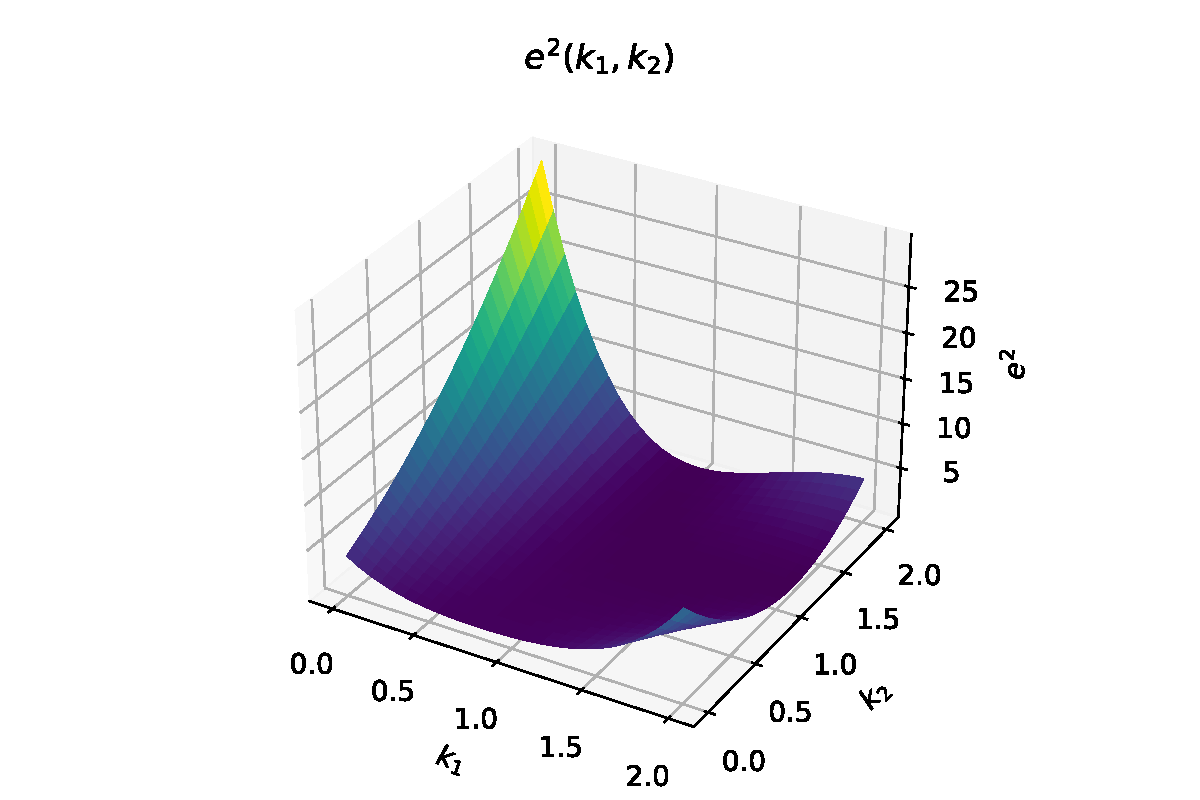
\includegraphics[
        %scale=1
        width=1\linewidth,]{figures/3d_plot_error_squared.pdf}
    \caption{\\$e^2(k_1, k_2)$}
    \label{fig:errorsquared3dplot}
\end{figure}
    


\begin{equation}\label{equ:expanded_drom_0000}
\begin{aligned}
f_{[dro]}(a) &= f(a, k_1=1.466, k_2=1.0012) = \\
&= 5.8710368 - 12.601424 a + 11.728 a^2 - 4 a^3
\end{aligned}
\end{equation}

 \begin{equation}\label{equ:equation_e_squared_k1k2}
            \begin{aligned}
            e^2(k_1, k_2) &=  \int_{1/2}^{1} rerr^2(x, k_1, k_2)\ dx = \\
            &= \int_{1/2}^{1} \left( \frac{f(x, k_1, k_2) - 1/x}{1/x} \right)^2 dx = \\
            &= \int_{1/2}^{1} \left( \frac{k_1 k_2 - 4(k_1^2 + k_2) x + 8 k_1 x^2 - 4 x^3 - 1/x}{1/x} \right)^2 dx = \\
            &= \frac{31 k_{1}^{4}}{10} - \frac{15 k_{1}^{3} k_{2}}{2} - \frac{21 k_{1}^{3}}{2} + \frac{14 k_{1}^{2} k_{2}^{2}}{3} + \frac{93 k_{1}^{2} k_{2}}{5} + \\ 
            &+ \frac{1339 k_{1}^{2}}{84} - \frac{15 k_{1} k_{2}^{2}}{2} - \frac{75 k_{1} k_{2}}{4} - \frac{375 k_{1}}{32} + \frac{31 k_{2}^{2}}{10} + \\ 
            &+ \frac{577 k_{2}}{84} + \frac{5507}{1440}
            \end{aligned}
        \end{equation}
        
We may want to know which are the optimal $k_1$ and $k_2$ such that:
\begin{equation}\label{equ:opt_k1_k2_eq}
(k_{1_{opt}}, k_{2_{opt}}): \min\{e^2(k_1, k_2)\}
\end{equation} 

For that the following system of equation (\ref{equ:opt_k1_k2_eq}) must be solved:
\begin{equation}\label{equ:opt_k1_k2_eq_partial}
\begin{cases}
\dfrac{\partial}{\partial k_1} e^2(k_1, k_2) = 0 \\
\dfrac{\partial}{\partial k_2} e^2(k_1, k_2) = 0
\end{cases}
\end{equation} 
\iffalse
$$
\begin{cases}
k_{1_{opt}} = 1.4567844114901045 \\
k_{2_{opt}} = 1.0009290026616422
\end{cases}
$$
\fi
which gives $(k_{1_{opt}} = 1.4567844114901045,\ k_{2_{opt}} = 1.0009290026616422)$, yielding a $36.4\%$ improvement over \cite{drom}'s $e^2$ figure. Figure \ref{fig:are_barplot} shows a comparison of the relative accuracy of the above mentioned functions and techniques w.r.t. $1/x$.

\begin{figure}
    \begin{center}
    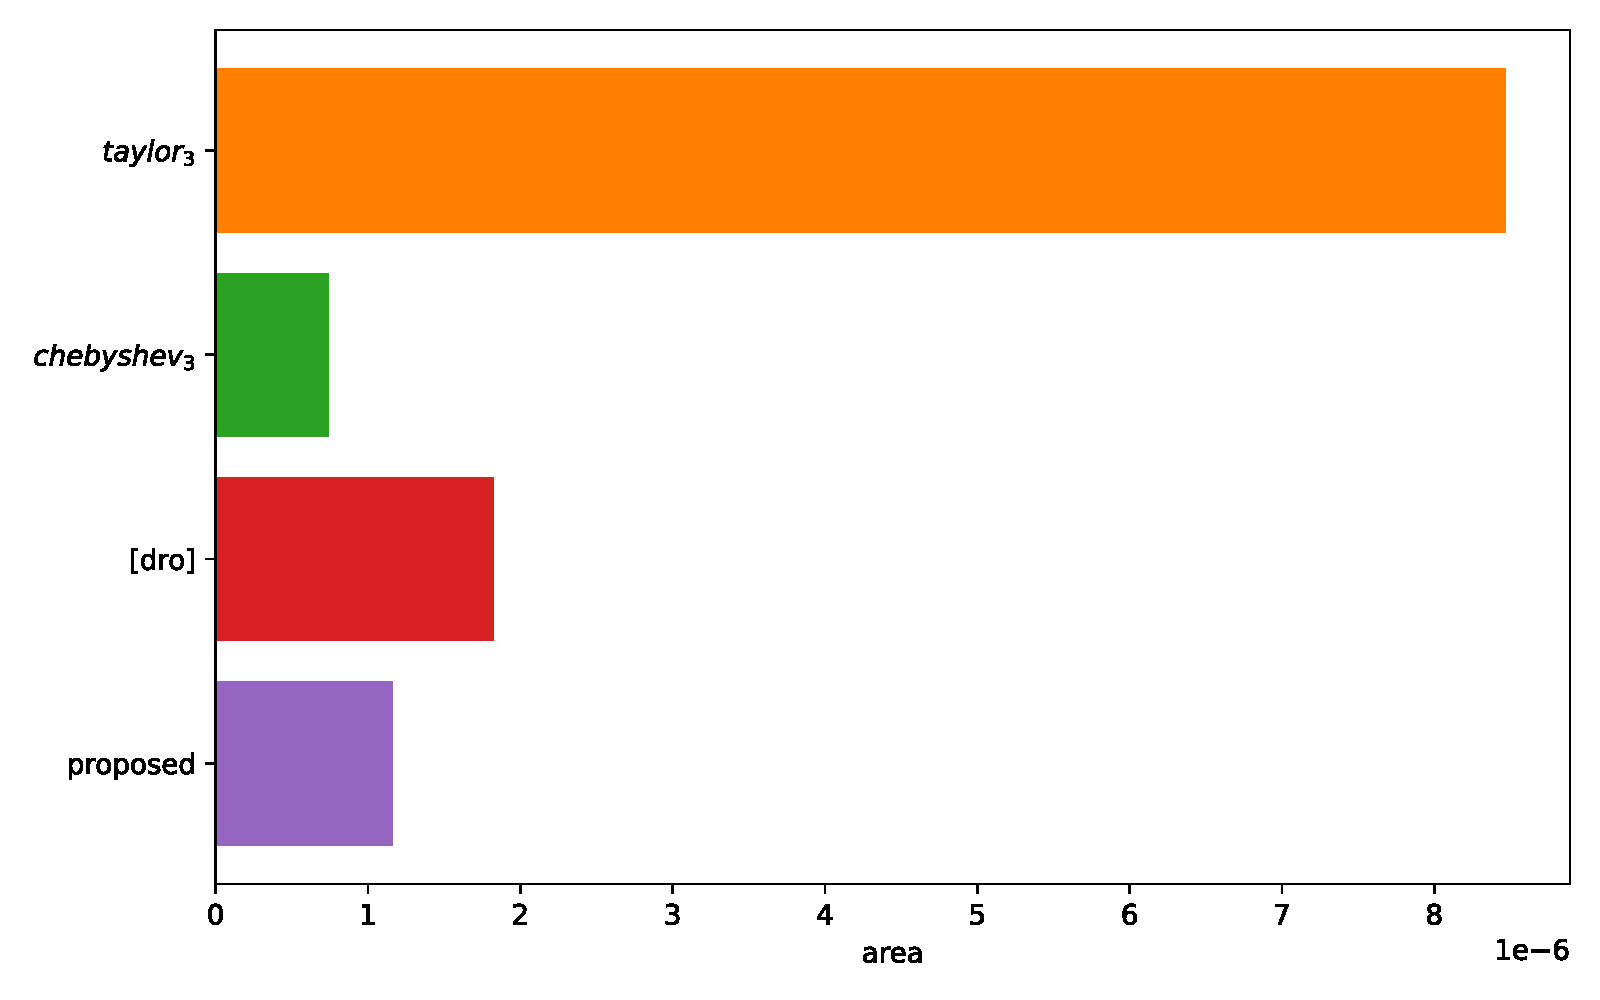
\includegraphics[width=0.4\textwidth]{figures/barplot_area_error.pdf}
    \caption{Barplot error area. $taylor_3$ vs $chebyshev_3$ vs \cite{drom} vs proposed}
    \label{fig:are_barplot}
    \end{center}
\end{figure}


With the best possible $k_1$ and $k_2$ constants set around our constraints -- i.e. (i) Chebyshev-like polynomial, and (ii) highest grade coefficient being a power of $2$\footnote{so that the bit shift trick can be performed, as opposed to yet another multiplication} -- we can now use the following routine to perform the approximated reciprocal, in a mostly accurate, yet efficient, way:

\begin{lstlisting}[label=alg:reciprocal_approx_modified_drom]
def reciprocal(a):
    b = k1_opt - a
    c = a * b
    d = k2_opt - c
    e = d * b
    out = e << 2
    return out
\end{lstlisting}

The bounds at each step of the algorithm can be easily determined, and consequently the correct fixed-point representation.

The only missing steps are the pre- and post-normalization of the input and, specularly, the output.
The input is a mantissa, hence $\in [1, 2)$: in order to fit the bound required by the algorithm, i.e. $[0.5, 1)$, dividing by $2$ is all that's needed. This is a simple right bit-shift. Similarly, a division by $2$ is required when the algorithm terminates to undo the effect of the pre-normalization and bring back the result into the desired bound.


Figure \ref{fig:reciprocal_unsigned_workflow} shows the flow of the procedure. 



\begin{itemize}
    \item \texttt{a} $\in [0.5, 1) \equiv A $ \dotfill \texttt{Fx<0, F>}
    \item \texttt{b} $\in (0.45702824, 0.95702824] $ \dotfill \texttt{Fx<0, F>}
    \item \texttt{c} $\in (0.45702824, 0.5307166278550605) $ \dotfill \texttt{Fx<0, 2F>}
    \item \texttt{d} $\in (0.47022002214493963, 0.54390841) $ \dotfill \texttt{Fx<0, 2F>}
    \item \texttt{e} $\in (0.24858150334349846, 0.4999731144222473) $ \dotfill \texttt{Fx<0, 3F>}
    \item \texttt{out} $\in (0.9943260133739938, 1.9998924576889892) $ \dotfill \texttt{Fx<1, 3F>}
\end{itemize}



    

\begin{figure}
    \centering
    \includegraphics[width=0.28\textwidth]{figures/reciprocal_unsigned.drawio.pdf}
    \caption{Reciprocal unsigned workflow}
    \label{fig:reciprocal_unsigned_workflow}
\end{figure}

\subsection{Ahead-of-time reciprocal}\label{aot_reciprocal_lut_technique}


The drawbacks of the solution illustrated in the previous section can be traded off for reduced result's precision at the benefit of a noticeble cut of implementation complexity.
That is where Ahead Of Time computation of the reciprocate comes into play: the idea being -- everything but novel -- rather than working out the reciprocate at run time, using dedicated, potentially bulky hardware multiplier instances, pre-computed results stored somewhere are retrieved and used.
The concept of Ahead Of Time (AOT) reciprocal computation is put into practice by means of look-up tables. This Look Up Table will take $N$ bits representing the $N$ most significant bits of the fraction and will output the $M$ most significant bits of the reciprocate of the input.

\begin{figure}[h!]
    \begin{center}
    \includegraphics[width=1\textwidth]{figures/lut.drawio.pdf}
    \caption{Look Up Table example, taking P$\langle 16,1 \rangle(0x71c0)$'s mantissa as input}
    \label{fig:lut_drawio_example}
    \end{center}
\end{figure}

With reference to the same posit, $P\langle 16,1 \rangle(0x71c0)$, figure \ref{fig:lut_drawio_example} gives a better idea of the mechanism: the posit's fraction field is first (extended to | trimmed at) $N$ bits; secondly the value represented by those bits is used to address the element in the Look Up Table corresponding to the $M$ most significant bits of the reciprocate of the full input mantissa.

Using a Look Up Table has the indirect added benefit of providing the designer an additional degree of freedom: $N$ and $M$ can be set independently and arbitrarily to better fit the best precision-to-footprint ratio.


\subsection{Newton-Raphson}\label{Newton_Raphson}


In numerical analysis, the Newton–Raphson method is a root-finding algorithm which produces successively better approximations to the roots of a real-valued function. The most basic version starts with a single-variable function $f$ defined for a real variable $x$, the function's derivative $f'$, and an initial guess $x_0$ for a root of $f$.
If the function satisfies sufficient assumptions and the initial guess is close, then
$$
x_{1} = x_0 - \frac{f(x_0)}{f'(x_0)}
$$
or more broadly,
\begin{equation}\label{equ:newon_raphson_generalized_equation}
x_{n+1} = x_n - \frac{f(x_n)}{f'(x_n)}
\end{equation}

This technique can be exploited to solve the problem of interest by noticing that if we consider a function whose root is such that $x = 1/n$, e.g.
\begin{equation}
f(x) = \frac{1}{x} - n
\end{equation}
with derivative
$$
f'(x) = -\frac{1}{x^2}
$$
where $n$ is the number whose reciprocate we are after and $x$ the reciprocate itself, the Newton Raphson method gives
\begin{equation}
\begin{aligned}
x_{n+1} &= x_n - \frac{f(x_n)}{f'(x_n)} = \\
& = x_n - \frac{\dfrac{1}{x_n} - n}{-\dfrac{1}{x_n^2}} = \\
& = x_n\ (2 - n \cdot x_n)
\end{aligned}
\end{equation}
which yields a valid approximation so long as the initial guess $x_0 \in (0, 2/n)$, as to not make the iteration diverge.


